\chapter{Introdução}

\indent Em ciências aplicadas, ao nos depararmos com uma determinada coisa a ser
estudada, a pergunta imediata é: como estudar tal coisa? Em problemas geofísicos,
essa coisa é, em geral, um sistema físico. O procedimento científico utilizado
para estudá-lo começa com a realização de observações (medições) de uma
determinada grandeza física que, supostamente, seja causada pelo sistema físico.
\\
\indent Exemplos de sistemas físicos encontrados na geofísica são:

\begin{itemize}
    \item{Propagação de ondas elásticas: sísmica (Figura \ref{system-seismic})}
    \item{Gravitação: gravimetria (Figura \ref{system-grav})}
    \item{Difusão de correntes elétricas: SEV (Figura \ref{system-sev})}
\end{itemize}

\begin{figure}
    \centering
    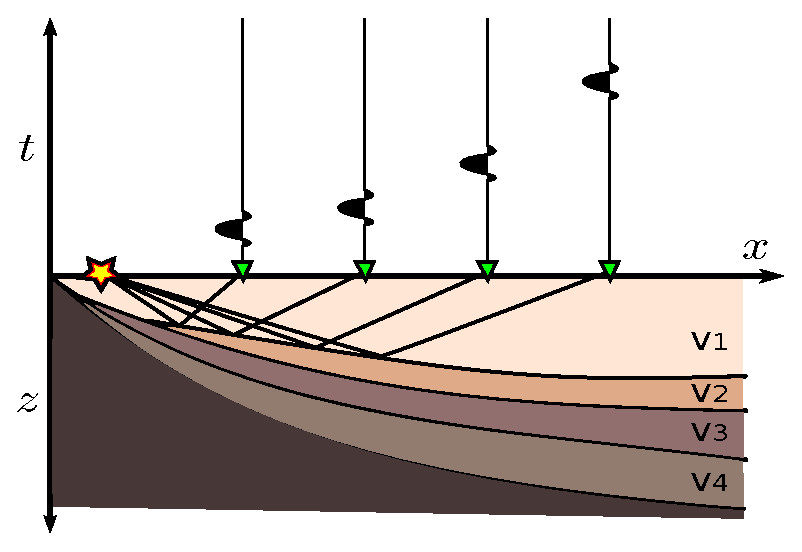
\includegraphics[scale=1]{../figs/system-seismic.eps}
    \caption{Exemplo de sistema físico que caracteriza uma aquisição sísmica.
        Neste caso o sistema envolve ondas sísmicas que se propagam em meios com
        diferentes velocidades. A grandeza física que podemos observar (medir)
        é o deslocamento dos sismômetros (neste caso somente na vertical).
        Estas observações são tipicamente dispostas em um sismograma.}
    \label{system-seismic}
\end{figure}

\begin{figure}
    \centering
    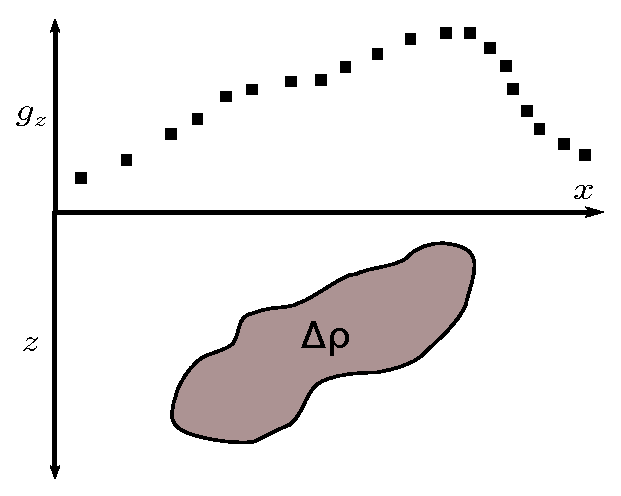
\includegraphics[scale=1]{../figs/system-grav.eps}
    \caption{Exemplo de sistema físico que caracteriza um levantamento
        gravimétrico. Neste caso o sistema envolve o efeito gravitacional
        causado por um contraste de densidade anômalo. A grandeza física que
        podemos observar (medir) é a anomalia da gravidade.}
    \label{system-grav}
\end{figure}

\begin{figure}
    \centering
    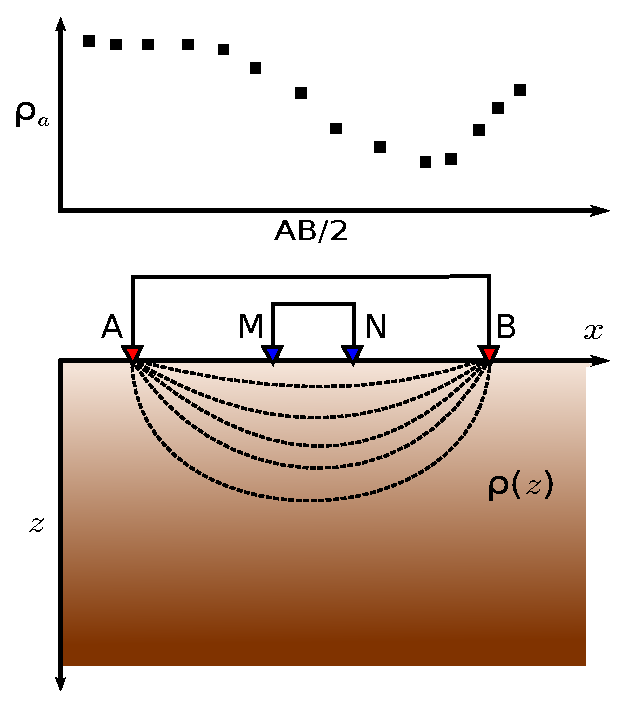
\includegraphics[scale=1]{../figs/system-sev.eps}
    \caption{Exemplo de sistema físico que caracteriza uma sondagem elétrica
        vertical (SEV). Neste caso o sistema envolve a condução de correntes
        elétricas em meios com diferentes resistividades elétricas ($\rho$).
        A grandeza física que podemos observar (medir) é diferência de potencial
        elétrico entre os eletrodos M e N. Esta grandeza é geralmente convertida
        para resistividade aparente ($\rho_a$).}
    \label{system-sev}
\end{figure}

\indent Uma vez que não conhecemos o sistema físico, a única coisa que temos são as
observações (dados observados). Contudo, embora o sistema físico seja
desconhecido, alguma informação adicional (em geral proporcionada pela geologia)
nos fornece um conjunto de hipóteses.
\\
Exemplos de hipóteses (sem dados observados e nem dados preditos)
\\
\indent Isso nos leva a seguinte pergunta: como testar se as observações podem ser
explicadas por uma determinada hipótese? Para responder esta pergunta,
precisamos ser capazes de calcular os dados preditos pela hipótese em questão.
\\
Exemplos de hipóteses e os respectivos dados preditos (sem dados observados)
\\
\indent Matematicamente, isso significa que precisamos encontrar uma função que
relaciona a hipótese aos dados preditos.

\begin{figure}[!htb]
  \centering
    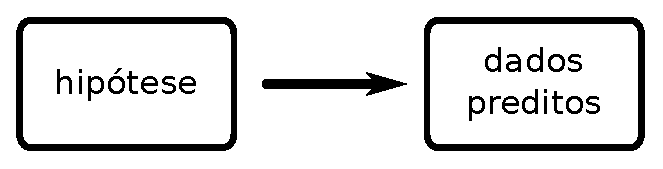
\includegraphics[scale=1]{../figs/hipotese-preditos.eps}
  %\caption{}
  \label{hipotese-preditos}
\end{figure}

Uma função é descrita em termos de parâmetros:
\\
Exemplos de funções
\\
\indent Portanto, calcular os dados preditos por uma determinada hipótese significa
encontrar uma função $f$ tal que:

\[
\text{dados preditos} = f(\text{hipótese}).
\]

\indent Para tanto, é preciso descrever a hipótese em termos de parâmetros
(parametrização), isto é:

\[
\text{dados preditos} = f(\text{parâmetros}).
\]

Exemplos de parametrização das hipóteses
\\
\indent O raciocínio desenvolvido acima nos permite definir um importante conceito:

\begin{quotation}
{\tt Estabelecer a relação funcional entre parâmetros (que descrevem uma hipótese)
e dados preditos é o que se co\-nhe\-ce como {\bf pro\-ble\-ma direto}.}
\end{quotation}

\indent Nesse sentido, dado um conjunto de parâmetros, é possível calcular os dados
preditos e isso nos permite testar se uma hipótese é capaz de explicar os dados
observados. Esse teste é feito por meio da comparação entre os dados observados
e os dados preditos por uma determinada hipótese. Se os dados preditos
reproduzem os dados observados, pode-se dizer que a hipótese explica os dados
observados e, portanto, é válida.
\\
Exemplos de hipóteses com os respectivos dados preditos, parâmetros e os dados observados
\\
\indent Nesse contexto, é possível podemos definir os seguintes conceitos importantes:

\begin{quotation}
{\tt Fornecer os parâmetros e comparar os respectivos dados preditos com os dados
observados é o que se conhece como {\bf mo\-de\-la\-gem direta}.}
\end{quotation}

e

\begin{quotation}
{\tt Estimar os parâmetros automaticamente, de forma que os dados preditos sejam os
mais próximos possíveis aos dados observados, é conhecido como {\bf problema inverso}.}
\end{quotation}

Figuras das setinhas
